\chapter{Míra souvislosti grafu}

\begin{definice}
	Graf je \textbf{souvislý} pokud jsou každé dva vrcholy spojené cestou, jinak je graf \textbf{nesouvislý} a je rozložen na aspoň dvě \textbf{komponenty souvislosti}.
\end{definice}

Nyní budeme zkoumat jak moc je graf odolný proti rozpadnutí po odebrání hrany nebo vrcholu.

\begin{definice}
	\textbf{Hranovým řez} v grafu $G = (V,E)$ je množina hran $F \subseteq E$ taková, že graf $G - F = (V, E \setminus F)$ je nesouvislý. (Také se někdy nazývá jako \textbf{separátor}.)
\end{definice}

\begin{definice}
	\textbf{Vrcholovým řezem} v grafu $G = (V,E)$ je množina vrcholů $A \subseteq V$ taková, že graf $G - A = (V \setminus A, E \cap \binom{V \setminus A}{2})$ je nesouvislý.
\end{definice}

\begin{definice}
	\textbf{Hranová souvislost} grafu $G = (V,E)$ je
	
	$$
	k_{e}(G) =
	\left\{
	\begin{array}{ll}
		\min\{|F|: F \text{ je hranový řez v }G \} \\
		k_{e}(G) = 1 \text{ pokud } G \equiv K_{1}
	\end{array}
	\right.
	$$
\end{definice}

\begin{definice}
	\textbf{Vrcholová souvislost} grafu $G = (V,E)$ je
	
	$$
	k_{v}(G) =
	\left\{
	\begin{array}{ll}
		\min\{|A|: A \text{ je vrcholový řez v }G \} \\ 
		k_{v}(G) = 1 \text{ pokud } G \equiv K_{1} \\
		k_{v}(G) = n-1 \text{ pokud } G \equiv K_{n}, n \geq 2
	\end{array}
	\right.
	$$
\end{definice}

Nesouvislé grafy mají vrcholovou i hranobvou souvislost 0. 

\begin{definice}
	Pro $r \in \mathbb{N}_{0}$ je graf \textbf{hranově $r$-souvislý}, pokud $k_{e}(G) \geq r$.
\end{definice}

\begin{definice}
	Pro $r \in \mathbb{N}_{0}$ je graf \textbf{vrcholově $r$-souvislý}, pokud $k_{v}(G) \geq r$.
\end{definice}

\begin{pozor}
	$\forall G = (V,E), G \neq K_{1}: k_{e}(G), k_{v}(G) \leq \min \{ \mathtt{deg}_{G}(v), v \in V \}$
\end{pozor}

\begin{lemma}
	$\forall G = (V,E) \forall e \in E: k_{e}(G) -1 \leq k_{e}(G-e) \leq k_{e}(G)$ Po odebrání hrany klesne hranová souvislost maximálně o 1.
\end{lemma}

\begin{proof}
	Empty.
\end{proof}

\begin{lemma}
	$\forall G = (V,E) \ \forall e \in E: k_{v}(G) -1 \leq k_{v}(G-e) \leq k_{v}(G)$ Po odebrání hrany klesne vrcholová souvislost maximálně o 1.
\end{lemma}

\begin{proof}
	Empty.
\end{proof}

\begin{dusl}
	$\forall G=(V,E): k_{v}(G) \leq k_{e}(G)$ Vrcholová souvislost je maximálně stejná jako hranová souvislost.
\end{dusl}

\begin{proof}
	Empty.
\end{proof}

Nerovnost může být ostrá. To lze vidět na příkaldu "motýlka". Lze vidět na obrázku \ref{motylek}.

\begin{figure}[!h]\centering
	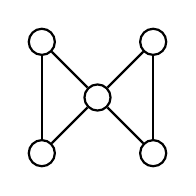
\begin{tikzpicture}[node distance={10mm}, thick, main/.style = {draw, circle}]
		\node[main] (1) {};
		\node[main] (2) [below right of=1] {};
		\node[main] (3) [below left of=1] {};
		\node[main] (4) [above right of=1] {};
		\node[main] (5) [above left of=1] {};
		\draw (1) -- (2);
		\draw (1) -- (3);
		\draw (1) -- (4);
		\draw (1) -- (5);
		\draw (4) -- (2);
		\draw (5) -- (3);
	\end{tikzpicture}
	\label{motylek}
	\caption{Graf "motýlek".}
\end{figure}

\begin{veta}[Ford-Fulkersonova věta]
	$\forall G \ \forall t \in \mathbb{N}: k_{e} \geq t \Leftrightarrow$ mezi každými $2$ vrcholy grafu $G$ $\exists$ $\geq t$ hranově disjunktních cest.
\end{veta}

\begin{proof}
	Empty.
\end{proof}

Varianat Fordovy-Fulkersonovy věty platí i pro vrcholovou souvislost. Tyto věty jsou známé také jako Mengerovy věty.

\begin{veta}[Mengerova věta]
	$\forall G \ \forall t \in \mathbb{N}: k_{e}(G) \geq t \Leftrightarrow$ mezi každými $2$ vrcholy grafu $G$ $\exists$ $\geq t$ vrcholově disjunktních cest (mimo $u,v$).
\end{veta}

\begin{proof}
	Empty.
\end{proof}

Jelikož lze zjistit tok maximální velikost v polynomiálním čase, tak máme algoritmus na zjištení $k_{e}(G), k_{v}(G)$ také v polynomiálním čase.

\section{2-souvislost podrobněji}

\begin{definice}
	Hranový řez velikosti $1$ se nazývá \textbf{most} a vrcholový řez velikosti  $1$ se nazývá \textbf{artikulace}.
\end{definice}

Pro graf $G=(V,E)$ s $e \in E$ označme $C \div e$ graf vzniklýz $G$ operací \textbf{podrozdělení hrany} $e$ na cestu délky $2$.

\begin{lemma}
	Pro každý graf $G=(V,E)$ a pro každou hranu $e \in E$ platí: $G$ je vrcholově $2$-souvislý $\Leftrightarrow G \div e$ je vrcholově $2$-souvislý.
\end{lemma}

\begin{proof}
	Empty.
\end{proof}

\begin{veta}[Ušaté lemma]
	Graf $G$ je vrcholově $2$-souvislý $\Leftrightarrow G$ lze vytvořit z $K_{3}$ operacemi přidávání a podroz-\newline dělování hran. Proč "Ušaté lemma"? Přidání hrany a její podrozdělení odpovídám přidání cesty mezi 2 vrcholy (="přiepení ucha").
\end{veta}

\begin{veta}[Alternativní znění]
	$G$ je vrcholově $2$-souvislý $\Leftrightarrow G$ lze vytvořit z cyklu přidá-\newline váním uší, protože přidávání ucha lze symulovat přidáním hrany a jejím podrozdělení.
\end{veta}

\begin{proof}
	Empty.
\end{proof}
